\chapter{Requirements}
\label{chapter:requirements}

To design a solution, environment around the problem needs to be understood, specifically, stakeholders involved and what needs they have. This chapter explains several industrial use cases with aim to familiarize the reader with environment Contracting Service is tailored for, followed by concrete requirements of this solution. Since there are countless number of different use cases, not everything can be covered, especially because new applications are continuously emerging. Therefore, this solution needs to be flexible to cover most of the existing and future use cases.  

\section{Context}
\label{section:context}

This section describes three representative industrial use cases in order to help reader understand the range of applications. All use cases have a common core even though they seem very different from each other as it can be seen from the following text.

\subsection{Smart Crane}

KoneCranes have donated a smart crane to Aalto Industrial Campus as a tool for research. This crane is an indoor crane whose head (which carries the load) is mounted on rails allowing it to reach every position inside, crane is pictured on figure ~\ref{fig:KoneCranes-CraneK16052}. Following information was gathered through interviews with researchers and with KoneCranes and it will be used as a representative example for the rest of this work.

\begin{figure}[ht]
	\begin{center}
		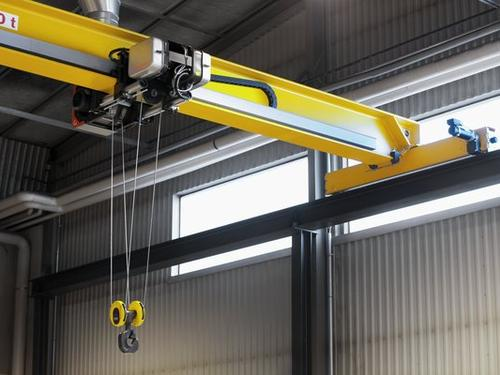
\includegraphics[width=\textwidth]{images/KoneCranes-CraneK16052}
		\caption{KoneCranes Indoor Crane (model K16052)}
		\label{fig:KoneCranes-CraneK16052}
	\end{center}
\end{figure}

This crane has many sensors attached to make it automated and smart as possible. These sensors
bring many features, namely {\bf load weighting} (which can also be used to detect
whether the crane is stuck somewhere), {\bf remote monitoring } of the position of the crane,
{\bf signaling} when some error or warning has occurred, {\bf live video feed } from camera attached
above the hook (at the moment, not used for automation but could be supported in the future,
for example, image processing to detect obstructions) and more.

There are multiple stakeholders in this ecosystem and all of them require some of the data
that Crane generates, although not all information should be available to them, only
the bare minimum that is required by their business. These stakeholders are KoneCranes, 
maintenance service (part of the KoneCranes) and users of the crane. Currently, KoneCranes has access to all the data Crane generates, but in order to 
increase security, this should not be the case.

\subsubsection{Maintenance}

Maintenance service makes use of usage data (alarms, usage parameters) to monitor and predict maintenance needs of the cranes. They also use the data together with the customer, in order to review their maintenance spend of the assets, study patterns to reveal relationships between variables and more. Following are some of the examples of use cases.

One part of the crane that needs to be changed most often are the breaks.
Breaks have limited number of uses and this number is approximately known
(there is a regulation in place that requires brakes to be changed regularly).
In order to determine whether the breaks needs changing or repair, maintenance service requires information about their usage. This information is provided by a pressure sensor installed on the breaks. How much pressure is needed to make the crane head stop is directly proportional to weight the crane is carrying which can then be used to calculate the wear of the breaks.

Large and expensive machines like this crane are under warranties and in order to determine whether the warranty is valid, maintenance service needs to know if the crane has been used in a proper way. Therefore, they need information coming from different sensors installed on the crane. These sensors include: 

\begin{enumerate}
	\setlength{\itemsep}{1pt}
	\item Pressure sensor on the crane head: determining whether the weight carried is in the recommended limits.  
	\item Temperature sensor on rails: when the crane head moves on the rails, friction generates heat and heat levels needs to be in a recommended limits in order for warranty to be valid.
	\item Pressure sensor on rails: determining whether they have been properly oiled.
	\item Humidity sensor: which determines whether the crane is kept in an environment suitable for it.
	\item Speed sensor: which determines whether the speed of crane head does not exceed recommended limits.
\end{enumerate}

Sensors listed are just several examples, and they can provide enough information for maintenance companies to determine whether the crane is being properly used. Crane sensors can also 
detect some irregularities and issue a warning (or error) directly to maintenance companies so that the problem can be addressed as fast as possible. 

Information like this should be disclosed to the maintenance service, while
restricting the access to data that can be used to infer the processes inside the factory. Examples include, position of the crane in a certain
point in time, or live feed from the camera mounted on the head.

\subsubsection{Users of the Crane}

Inside a factory there are different actors with different privileges. These actors can be roughly grouped in two categories: workers and managers. 
Worker operating the crane should have restricted access to data the crane operates. Information that he needs is tied to the current operation of the crane and some of the sensors that give that information are following. Position sensor, which tells him where the head of the crane is in space, and pressure sensor measuring the weight of the load. On the other hand, worker should not have information about the conditions of the brakes or temperature of the rails since it is of no use to him.

Managers responsible for multiple workers and machines should have access to all information related to operations of these machines. In that way, they can monitor their workers remotely, ensuring that everything is operating smoothly.

In the future, machine to machine communication will be utilized much more, for example, 
in a setting with two Cranes operating (automated, not by human) in the same room they 
should be able to signal to each other with their planned path in order to avoid collisions
and to optimize the process. In this way, need for a centralized control is eliminated (or at
least minimized).

\subsubsection{KoneCranes}

KoneCranes needs access to some of the data that Crane generates, in order to make product improvements, react to possible reliability problems and get better specification for new product generations, and adjust warranties.
They analyze all types of data that Crane generates including: 

\begin{enumerate}
	\setlength{\itemsep}{1pt}
	\item Manufacturing data: such as component lists and manufacturing dates.
	\item Usage data: including number of hours in operation, weights carried, mileage of the crane head and more
	\item Sensor data: such as vibrations and temperature
	\item Maintenance data: examples include maintenance task history, ordered materials and more.
\end{enumerate}

As mentioned, at the moment KoneCranes has access to all the data Crane generates and their customers are aware
of that. For privacy reasons, and in environment with multiple manufacturers, data access should be restricted to only what is needed for a specific role. 

\subsection{Smart Traffic}

Recently, smart traffic is emerging as promising trend with the idea to automate transportation of goods and people. Big corporations, such as Google, Tesla, Mercedes and Uber have already joined the race with their models but many technological, legal and business obstacles are holding back its deployment. Integration of these vehicles into regular, non-automated traffic is a big challenge since it needs to take into account human error and correct it if possible.

One interesting example are smart convoys, driver-less trucks transporting goods in a convoy. For this to be secure, communication between trucks needs to be in real-time so that all, for example, obstructions noticed by sensors on truck in front are conveyed to the rest in time to react (slowing down or avoiding obstruction). It is also very important that only authorized people have access to data convoy produces, because if something gets tampered with, human lives are at stake along with structural damages. 

For these security reasons not all stakeholders should have access to all the data but only to what is necessary for their operations. Stakeholders involved are: manufacturers; maintenance company; users; and third parties. Firstly, manufacturers should not have access to data that discloses anything that is confidential for truck users, for example, exact location of the convoy in any time because this information can be used to get insight into operations of users. Secondly, manufacturers might not want to give out all information to their users, either because of confidentiality or because it might discredit them. Thirdly, maintenance companies should have only information about the state of the parts of truck. How many times have the breaks been used, level of motor oil, gas and similar, which they need in order to schedule maintenance control. Finally, third parties could be any company, or public, that benefits from data these trucks produce and fit into business models of manufacturers or users. For example, traffic control application that provides information about how many convoys are on a particular road so that if the number is too high, traffic jams are expected.

\subsection{Connected Goods}

The  servitisation  of  physical  goods  will  be  of  strategic  importance  for the  manufacturing  industry, where instead of selling parts and machines it will be possible to sell engine hours, kilometers and similar. The vision here is that goods will remember how they were made and produce data throughout whole cycle of their usage, even giving insights into customer satisfaction with those goods. In this case, privacy is a big obstacle, because it is hard to assure customer that data you collected in their home or workspace is not going to be used by anybody they do not want to.

Consider a scenario where all goods in your apartment from carton of milk to air-conditioning are equipped with sensors. Milk carton might posses a heat sensor, which alerts when milk is being kept in a warm place for too long, labeling it as spoiled and ordering fresh one from a local marketplace. Same data can be used for statistical purposes by a third party, to determine, for example, how much milk is being wasted by a nation and use it to adjust size of milk cartons or predict peaks in milk consumption. With some more complex goods, such as air-conditioning, predictive maintenance can be realized with sensors that tell if a particular part is wearing off and alert maintenance service specified by user or manufacturer of that machine. Subset of the data generated by air-conditioning can be used by health organizations to determine whether people are living in unhealthy environments, for example, by checking the ratio between how many times air filters have been changed over hours of usage.

Scenarios described in previous paragraph are just few out of many possible ones and it is impossible to tell, which ones will be implemented. Although, we have to prepare for the future by designing a flexible system that can withstand rapid changes in the ecosystem.

\section{Contracting Service Requirements}

At this point, the environment Contracting Service is tailored for has been explained. It is clear from previous section that this solution requires different accounts for all actors involved according to their role. These roles are, roughly, be divided into three groups: Administrators, Manufacturers and Customers.

Remainder of this section is organized into four subsections. First subsection will give general requirements for this platform, spanning requirements regarding security, user interface design rules and functional requirements required for all roles. Following subsections will describe requirements for each role in the system, administrator, manufacturer and customer respectively.    

\subsection{General Requirements}

Following text will describe general requirements for this solution, drawn from the context explained in section ~\ref{section:context}. It will address requirements related to security, user experience and functional requirements not tied to any specific role.

\subsubsection{Security}
\fixme{Talk about general security especially of devices,Authentication}
\fixme{talk about most common attacks, like cross site request forgery}


\subsubsection{User Experience}
\fixme{ Niemens 10 rules of good design?}

\subsubsection{Functional Requirements}
\fixme{, some stuff like changing user info, checking user info, managing devices/policies for device or set of devices/machine }

\subsection{Administrator Requirements}

Administrator of the platform has the simplest role in the system, although he has big responsibility. He is a central, impartial authority that makes sure that the system is running smoothly. Apart from regular responsibilities of system administrator, he is \emph{required to create accounts for manufacturers} and manage them. 

This requirements comes from the fact that, in order to qualify as a manufacturer, you need to have a verified manufacturing company. In order to fully understand the need for this requirement, consider a scenario where everybody is allowed to create an account and pose as a manufacturer. This scenario introduces security concerns, such as a party acting as a manufacturer and assigning fictional devices to a customer, thus affecting customers view of the platform.

\subsection{Manufacturer Requirements}

Manufacturers of smart industrial machines have a central role in the whole ecosystem, they are the providers of the service of selling or lending machines. Therefore, their requirements are of great importance. They have all necessary information about machines they are manufacturing, thus, they should be the ones adding the machines to the system and assigning them to the customers. Following list will explain all of their requirements thoroughly:

\begin{enumerate}
	\setlength{\itemsep}{1pt}
	\item \textbf{\textit{Create customer accounts}}: Allowing anybody to create a customer account may create many empty accounts that are only taking space in the database. Furthermore, there is no use for them if they do not possess any machines. Therefore, when customers buy or lend a machine \emph{for the first time}, their accounts need to be created. Depending on the needs of the customer, opening multiple accounts should be possible. 

	\item \textbf{\textit{Managing templates}}: Almost every machine that is being produced is not one of a kind, it is made following a model. Manufacturers offer many different models to their customers, such as a smart crane pictured on figure ~\ref{fig:KoneCranes-CraneK16052} with model number K16052. Therefore, manufacturers need a way to define templates describing different models of their machines. These templates represent a simplified "digital twin" of a particular machine describing devices that are attached to it. This requirement consists of three smaller requirements:

	\begin{enumerate}
		\item \textbf{\textit{Add templates}}: Way to introduce new templates needs to be available.
		\item \textbf{\textit{Delete templates}}: Deleting faulty or outdated templates needs to be available.
		\item \textbf{\textit{View templates}}: Overview of all templates needs to be presented to manufacturer. 
	\end{enumerate}

	\item \textbf{\textit{Add machine through a template}}: When the necessary templates are added to the system, manufacturers should be able to instantiate them to create a machine and add it to the system. Adding machines following a template reduces error and work needed when inputing data for all devices for a machine.

	\item \textbf{\textit{Add custom machines}}: As mentioned in Managing templates, almost every machine is made using a template. Although, some machines are custom made on a request of the customer. These machines do not require a template because they are not being massively produced. Therefore, a way to add custom machines is required.

	\item \textbf{\textit{Remove and modify machines}}: For any machine, regardless of how it was inputed into system, there needs to be a way to remove them or to modify their contents.

	\item \textbf{\textit{Manage machines and devices}}: When all necessary machines are added to the system they need to be assigned to customers. It should only be possible to assign machines to the customers of a specific manufacturer (not the customers of different manufacturers). This requirement consists of three smaller requirements:
		\begin{enumerate}
			\item \textbf{\textit{Assign machine or device to customer}}: A way to assign a certain machine or device so it becomes visible to the customer needs to be available to the manufacturer.
			\item \textbf{\textit{Remove assignment of machine or device}}: Reverting the action of assigning a machine or device to customer needs to be provided in order to account for faulty assignments, or if the machine or device was lent for a certain period of time.
			\item \textbf{\textit{View assignments}}: In order to control which machines and devices are assigned to whom, an overview of assignments needs to be provided.
		\end{enumerate}
\end{enumerate}

\subsection{Customer Requirements}

Customer requirements are slightly more complicated that manufacturers. Only one account (or a fixed number) of accounts is not necessarily sufficient since the buyer of the machine is rarely the user of the machine. Inside every company there is a hierarchy of responsibilities, where different people are responsible for a subset of machines that the customer company owns. Therefore, it is necessary for customer to be able to create as many accounts as his business requires (this number can be zero). These accounts that a customer creates shall be referred as users in the remainder of this thesis. Following text will list customer requirements, followed by requirements that user shares with customer:

\begin{enumerate}
	\setlength{\itemsep}{1pt}
	\item \textbf{\textit{Create user accounts}}: As mentioned above, creation of user accounts is crucial in order to assign responsibilities for certain machines to several actors inside a company. These actors are some type of managers overlooking the machines they are responsible for.

	\item \textbf{\textit{Manage machines and devices}}: When all necessary machines are added to the system by manufacturers and assigned to customers, they need to be assigned to users responsible for them. In certain cases (for example, in a small company), customer retains all responsibility for machines and do not assign them to anyone else. This requirement consists of three smaller requirements:
		\begin{enumerate}
			\item \textbf{\textit{Assign machine or device to user}}: A way to assign a certain machine or device to the user needs to be available in order for the user to manage access to the machine or device.
			\item \textbf{\textit{Remove assignment of machine or device}}: Reverting the action of assigning a machine or device to the user needs to be provided in order to account for faulty assignments, or if the machine or device needs to be assigned to someone else.
			\item \textbf{\textit{View assignments}}: In order to control what machines or devices are assigned to whom, an overview of assignments needs to be provided.
		\end{enumerate}
\end{enumerate}

Requirements listed above are only for the customer. User requirements are similar to customer with the exception of creating additional accounts and assigning machines. Following list describes additional requirements of customers which are also all requirements of users:

\begin{enumerate}
	\setlength{\itemsep}{1pt}
	\item \textbf{\textit{Allow access to machine or device}}: Allowing customers to define who can access the data their machines produce is highly important. Customer should be able to define access for the whole machine or parts of the machine by controlling access to particular devices, such as a temperature sensor on crane previously described in section ~\ref{section:context}. Additionally, customer needs to be able to define duration and direction of the communication, explained bellow:
		\begin{itemize}
			\item \textbf{\textit{Duration}}: Duration of allowed access is defined by start and end date.
			\item \textbf{\textit{Direction of communication}}: Communication from customer device to the target means that only customer device can send data to the target while rejecting all requests from the target. Opposite direction means that the target can only send requests to the customer device, such request typically give instructions to the device. Allowing flexibility to define direction of communication is highly important to the customer.
		\end{itemize}

	\item \textbf{\textit{Remove previously allowed access to machine or device}}: A way to revert action of allowing access to a machine or device needs to be provided. 
		
	\item \textbf{\textit{View who has access to your machines}}: In order for customer to be fully aware of who has access to their machines, and overview needs to be provided.

\end{enumerate}

